% 第 2 章续：第三批图片，2.55--2.64。
\problem[$\ast\ast$；数值实验]{2.55}
利用“摇摆狗尾”方法，求出谐振子的基态能级，并保留 5 位有效数字。也就是说，用数值法求解方程（2.73），通过不断改变 $K$ 值，直到 $\xi$ 很大时，能得到一个趋于零的波函数。在 Mathematica 中，适当的输入程序语句为：
\begingroup\small
\begin{verbatim}
Plot[
  Evaluate[
    u[x] /.
      NDSolve[
        {u''[x] - (x^2 - K)*u[x] == 0,
         u[0] == 1, u'[0] == 0},
        u[x], {x, 0, b}
      ]
  ],
  {x, a, b}, PlotRange -> {c, d}
]
\end{verbatim}
\endgroup
（这里 $(a,b)$ 是图中水平方向取值范围，$(c,d)$ 是竖直方向的取值范围——起始值分别是：$a=0$，$b=10$，$c=-10$，$d=10$。）我们知道正确解满足 $K=2n+1$，所以可以从“猜测的值”$K=0.9$ 开始。注意观察波函数“尾部”的变化行为。再尝试 $K=1.1$，注意“尾部”的快速翻转。正确解就位于这两个值之间的某处。通过调整使两端的 $K$ 值差越来越小，使波函数尾部归零。这样做的时候，你也可以调整 $a$、$b$、$c$ 和 $d$ 的值，使零点出现在交叉点。
\vfill

\problem[数值实验]{2.56}
利用习题 2.55 中的“摇摆狗”方法求出谐振子的前 3 个激发态的能级（保留五位有效数字）。对第一（和第三）激发态需要设定 $u(0)=0$，$u'(0)=1$。
\vfill

\problem[数值实验]{2.57}
利用“摇摆狗”方法求出无限深方势阱中的前 4 个能级（保留五位有效数字）。提示：参看习题 2.55，对微分方程做适当改变。本题需要寻找的条件是 $u(1)=0$。
\vfill

\problem{2.58}
在单价金属固体中，每个原子的一个电子在固体中自由运动。是什么把固体结合在一起的？为何他们不散落成一堆单独的原子？显然是聚集结构的能量一定比每个孤立原子的总能量小。本题目给出关于金属结合的一个粗略但具有启发性的解释。
\begin{enumerate}
\item 把孤立金属原子看成是其一个电子处在宽度为 $a$ 的无限深方势阱中的基态（见下图（a），原书图 2.23a），估计 $N$ 个孤立原子的能量。
\item 当这些原子聚集一起形成金属，可以看作是 $N$ 个电子位于宽度为 $Na$ 的无限深势阱中运动（见下图（b），原书图 2.23b）。由于泡利不相容原理（将在第 5 章讨论），每个允许的能级只能有一个电子（如果考虑自旋，为两个电子；先忽略自旋）。这样一个系统的最低能量是多少？
\item 上述两种情况下的能量差就是金属的内聚能（cohesive energy）——也就是把金属撕裂成孤立原子所需要的能量。在 $N$ 很大的极限情况下，求出每个原子的内聚能。
\item 金属中典型原子间的距离是几个埃（比如，$a\approx4\,\text{\AA}$），在此模型中每个原子的内聚能的数值是多少（测量值在 $2\sim4\,\mathrm{eV}$ 的范围内）？
\end{enumerate}
\begin{center}
% 原书图 2.23 的定性重绘：孤立的 N 个阱与一个共同势阱。
\begin{tikzpicture}[x=0.85cm,y=0.6cm,>=Stealth,font=\small]
\foreach \x in {0,1.5,3,6.5}{
  \draw[thick] (\x,2.1)--(\x,0)--(\x+0.95,0)--(\x+0.95,2.1);
  \draw (\x+0.48,0.08) circle (0.065);
}
\node at (5.15,0.8) {$\cdots$};
\draw[|<->|] (0,-0.4)--(0.95,-0.4) node[midway,below] {$a$};
\node at (3.75,-0.65) {（a）};
\begin{scope}[yshift=-3.2cm]
\draw[thick] (0,2.1)--(0,0)--(7.45,0)--(7.45,2.1);
\foreach \x in {0.3,1.05,1.8,2.55,3.3,5.2,5.95,6.7}{
  \draw (\x,0.08) circle (0.065);
}
\node at (4.2,0.12) {$\cdots$};
\draw[|<->|] (0,-0.4)--(7.45,-0.4) node[midway,below] {$Na$};
\node at (3.75,-1.2) {（b）};
\end{scope}
\end{tikzpicture}

\par\smallskip{\small 习题 2.58 图：（a）独立势阱；（b）宽度为 $Na$ 的共同势阱}
\end{center}
\vfill

\problem[$\ast$；数值实验]{2.59}
\textbf{“弹跳球”。}假设
\[
V(x)=\begin{cases}mgx,&x>0,\\\infty,&x\leq0.\end{cases}
\]
\begin{enumerate}
\item 求解该势的定态薛定谔方程。提示：首先把方程转换成无量纲形式：
\[
-y''(z)+zy(z)=\varepsilon y(z),
\]
通过令 $z=\alpha x$ 和 $y(z)=(1/\sqrt{\alpha})\psi(x)$（$\sqrt{\alpha}$ 使得若 $\psi(x)$ 对于 $x$ 是归一化的，则 $y(z)$ 对于 $z$ 也是归一化的）。常数 $\alpha$ 和 $\varepsilon$ 的值是多少？事实上，也可以令 $\alpha\to1$——这等同于方便选择一个长度单位。求出方程的一般解（Mathematica 中的 \texttt{DSolve} 指令可以实现）。当然，结果是两个（可能是不熟悉的）波函数的线性组合。在 $-15<z<5$ 区间内，画出两个波函数。其中的一个波函数在 $z$ 较大时明显地不趋于零（更确切地说，它不可以归一化），因此，舍弃它。$\varepsilon$ 的允许值（也是 $E$ 的允许值）由条件 $\psi(0)=0$ 确定。数值计算基态能量 $\varepsilon_1$ 和第 10 个能级 $\varepsilon_{10}$（Mathematica 中的 \texttt{FindRoot} 指令可以实现）。给出其相应的归一化因子。在 $0\leq x\leq16$ 区间内，画出 $\psi_1(x)$ 和 $\psi_{10}(x)$。仅仅作为检验，确定 $\psi_1(x)$ 和 $\psi_{10}(x)$ 是正交的。
\item 对于这两个状态，求出其不确定度 $\sigma_x$ 和 $\sigma_p$，并验证符合不确定原理。
\item 求位于高度 $x$ 位置的 $\dd x$ 区间内，发现该球的几率是 $\rho_Q(x)\,\dd x=|\psi(x)|^2\,\dd x$。最接近的经典类比是弹性球在高度 $x$ 位置处 $\dd x$ 区间所经历时间的分数（见习题 1.11）。证明其为
\[
\rho_C(x)\,\dd x=\frac{mg}{2\sqrt{E(E-mgx)}}\,\dd x,
\]
或者，以我们的单位（$\alpha=1$），
\[
\rho_C(x)=\frac{1}{2\sqrt{\varepsilon(\varepsilon-x)}}.
\]
在 $0\leq x\leq12.5$ 区间内，画出态 $\psi_{10}(x)$ 的 $\rho_Q(x)$ 和 $\rho_C(x)$ 的叠加图形（Mathematica 中的 \texttt{Show} 命令），并讨论你的结果。
\end{enumerate}
\vfill

\problem[$\ast\ast\ast$；数值实验]{2.60}
\begingroup\small
\setlength{\abovedisplayskip}{5pt}
\setlength{\belowdisplayskip}{5pt}
\textbf{$1/x^2$ 势。}假设
\[
V(x)=\begin{cases}-\alpha/x^2,&x>0,\\\infty,&x\leq0,\end{cases}
\]
这里 $\alpha$ 是具有适当量纲的正常数。我们希望找到其束缚态——求解能量为负值的（$E<0$）定态薛定谔方程：
\[
-\frac{\hbar^2}{2m}\frac{\dd^2\psi}{\dd x^2}-\frac{\alpha}{x^2}\psi=E\psi.
\]
\begin{enumerate}
\item 讨论基态能量 $E_0$：从量纲的角度证明，不可能存在 $E_0$ 的公式——无法（从可以利用的常数 $m$、$\hbar$ 和 $\alpha$）来构造一个具有能量单位的物理量。
\item 简便起见，式（2.190）重写为
\[
\frac{\dd^2\psi}{\dd x^2}+\frac{\beta}{x^2}\psi=\kappa^2\psi,
\qquad\text{这里 }\beta=\frac{2m\alpha}{\hbar^2},\quad
\kappa=\frac{\sqrt{-2mE}}{\hbar}.
\]
证明：如果 $\psi(x)$ 满足上述方程，能量为 $E$，那么，对任意的正数 $\lambda$，$\psi(\lambda x)$ 也一样满足，且能量为 $E'=\lambda^2E$。（这是个灾难。如果真的存在解，那么也就存在对任何负能量都成立的一个解。与我们遇到过的方势阱、谐振子和所有的其他势阱不一样，不存在离散的许可状态——且没有基态。一个没有最低的能量允许值的基态的系统——将是极其不稳定，级联式的能级下降，在下落时释放无限的能量。它也许可以解决我们的能源问题，但在这个过程中我们都将被灼伤。）好的，也许根本就没有解……
\item 证明（利用计算机来解决其余部分）
\[
\psi_\kappa(x)=A\sqrt{x}\,K_{\mathrm{i}g}(\kappa x)
\]
满足式（2.191）（这里 $K_{\mathrm{i}g}$ 是 $\mathrm{i}g$ 阶修正的贝塞耳函数，且 $g=\sqrt{\beta-1/4}$）。对 $g=4$，画出该波函数（图中你不妨令 $\kappa=1$，这只是设置长度的标度）。注意当 $x\to0$ 和 $x\to\infty$ 时，$\psi_\kappa$ 趋近零，所以它是可归一化的：确定 $A$ 的值。\footnote{只要 $g$ 是实数——也就是说，在 $\beta>1/4$ 的条件下，$\psi_\kappa(x)$ 就是可归一化的。}前述的节点数等于能量较低的状态数这一旧规则会变得如何？无论能量大小（即 $\kappa$ 的大小），这个函数有无限个节点，我想这是一致的，因为对任意的 $E$，都存在无限多的比其能量更低的态。
\item 这个势函数几乎混淆了我们所期望的一切。问题是这个势在 $x\to0$ 时，变化得太剧烈。如果你把这个“砖墙”移动一点，
\[
V(x)=\begin{cases}-\alpha/x^2,&x>\epsilon>0,\\\infty,&x\leq\epsilon,\end{cases}
\]
突然它们就变得正常了。对于 $g=4$ 和 $\epsilon=1$，在 $x=0$ 至 $x=6$ 范围内画出基态波函数（你首先需要确定合适的 $\kappa$ 值），注意我们引入了具有长度的量纲的新参数（$\epsilon$），因此，在（a）中的争论不在讨论范围之内。证明：对无量纲变量 $\beta$ 的一些函数 $f$，基态能具有形式
\[
E_0=-\frac{\alpha}{\epsilon^2}f(\beta).
\]
\end{enumerate}
\endgroup
\vfill

\problem[$\ast\ast\ast$；数值实验]{2.61}
\begingroup\small
\setlength{\abovedisplayskip}{4pt}
\setlength{\belowdisplayskip}{4pt}
获得势阱能级允许值的一种数值方法是，通过变量 $x$ 的离散化把薛定谔方程变成矩阵方程。在等间距的点 $\{x_j\}$ 中划分出相关间隔，$x_{j+1}-x_j=\Delta x$，令 $\psi_j=\psi(x_j)$（同样，$V_j=V(x_j)$），那么
\[
\frac{\dd\psi}{\dd x}\approx\frac{\psi_{j+1}-\psi_j}{\Delta x},\qquad
\frac{\dd^2\psi}{\dd x^2}\approx
\frac{(\psi_{j+1}-\psi_j)-(\psi_j-\psi_{j-1})}{(\Delta x)^2}
=\frac{\psi_{j+1}-2\psi_j+\psi_{j-1}}{(\Delta x)^2}.
\]
（随着 $\Delta x$ 的减少，这种近似将逐步改善。）离散的薛定谔方程是
\[
-\frac{\hbar^2}{2m}\left(\frac{\psi_{j+1}-2\psi_j+\psi_{j-1}}{(\Delta x)^2}\right)
+V_j\psi_j=E\psi_j,
\]
或者
\[
-\lambda\psi_{j+1}+(2\lambda+V_j)\psi_j-\lambda\psi_{j-1}=E\psi_j,
\qquad\text{这里 }\lambda=\frac{\hbar^2}{2m(\Delta x)^2}.
\]
矩阵形式
\[
\boldsymbol H\boldsymbol\Psi=E\boldsymbol\Psi.
\]
这里（令 $v_j=V_j/\lambda$）
\[
\boldsymbol H=\lambda
\begin{pmatrix}
\ddots&&&&&\\
&-1&2+v_{j-1}&-1&0&0\\
&0&-1&2+v_j&-1&0\\
&0&0&-1&2+v_{j+1}&-1\\
&&&&&\ddots
\end{pmatrix},
\qquad
\boldsymbol\Psi=\begin{pmatrix}\vdots\\\psi_{j-1}\\\psi_j\\\psi_{j+1}\\\vdots\end{pmatrix}.
\]
\textbf{整理注：}原图式（2.199）的矩阵前未写整体因子 $\lambda$；此处按式（2.197）补入，使矩阵方程与差分方程、能量量纲一致。

（下面将会看到，$H$ 的左上角和右下角是什么依赖于边界条件。）很明显，能量允许值是矩阵 $H$ 的本征值（或者说，$\Delta x\to0$ 的极限）。

将这种方法应用于无限深方势阱。把 $0\leq x\leq a$ 区间分成 $N+1$ 个相等的部分（所以 $\Delta x=a/(N+1)$），令 $x_0=0$ 和 $x_{N+1}=a$。边界条件 $\psi_0=\psi_{N+1}=0$，有
\[
\boldsymbol\Psi=\begin{pmatrix}\psi_1\\\vdots\\\psi_N\end{pmatrix}.
\]
\begin{enumerate}
\item 对 $N=1$、$N=2$ 和 $N=3$，构造 $H$ 的 $N\times N$ 矩阵。（对于特殊情况 $j=1$ 和 $j=N$，确保能够正确地表示出式（2.197）。）
\item 对这 3 种情况，“手动”求出 $H$ 的本征值，并与精确的能级允许值（式（2.30））作比较。
\item 对 $N=10$ 和 $N=100$，利用计算机数值求解出最低的 5 个能级本征值（Mathematica 中 \texttt{Eigenvalues} 软件包可以处理这个问题），并与精确解比较。
\item 画出（“手动”）$N=1$、$N=2$ 和 $N=3$ 时的本征矢，用计算机（\texttt{Eigenvectors} 软件包）画出 $N=10$ 和 $N=100$ 时的前 3 个本征矢。
\end{enumerate}
\endgroup
\vfill

\problem[$\ast\ast$；数值实验]{2.62}
假设无限深方势阱的底部不是平坦的（$V(x)=0$），而是
\[
V(x)=500V_0\sin\left(\frac{\pi x}{a}\right),
\qquad\text{这里 }V_0=\frac{\hbar^2}{2ma^2}.
\]
使用习题 2.61 中的数值方法求出其前 3 个能量允许值，并画出其相应的波函数（取 $N=100$）。
\vfill

\problem{2.63}
\begingroup\small
\setlength{\abovedisplayskip}{4pt}
\setlength{\belowdisplayskip}{4pt}
玻尔兹曼方程
\[
P(n)=\frac{1}{Z}\mathrm{e}^{-\beta E_n},\qquad
Z=\sum_n\mathrm{e}^{-\beta E_n},\qquad\beta\equiv\frac{1}{k_{\mathrm B}T},
\]
给出系统在温度为 $T$ 时，处在状态 $n$（能量为 $E_n$）的几率（$k_{\mathrm B}$ 是玻尔兹曼常量）。注释：这里的几率指的是随机热分布，与量子的不确定没有任何关系。只有在能量 $E_n$ 量子化情况下，该问题才涉及量子力学。
\begin{enumerate}
\item 说明系统能量的热平均可以表示为
\[
\overline E=\sum_n E_nP(n)=-\frac{\partial}{\partial\beta}\ln Z.
\]
\item 对于简单的量子谐振子，指标 $n$ 就是量子数，且 $E_n=(n+1/2)\hbar\omega$。证明在这种情况下，配分函数（partition function）$Z$ 为
\[
Z=\frac{\mathrm{e}^{-\beta\hbar\omega/2}}{1-\mathrm{e}^{-\beta\hbar\omega}}.
\]
你需要对一个几何级数序列求和。顺便提及，对于经典谐振子，可以证明 $Z_{\text{经典}}=2\pi/(\omega\beta)$。
\item 利用（a）和（b）的结果，证明：对于量子谐振子
\[
\overline E=\left(\frac{\hbar\omega}{2}\right)
\frac{1+\mathrm{e}^{-\beta\hbar\omega}}{1-\mathrm{e}^{-\beta\hbar\omega}}.
\]
对经典谐振子，同样的推理可以得到 $\overline E_{\text{经典}}=1/\beta=k_{\mathrm B}T$。
\item 由 $N$ 个原子组成的晶体可以看成 $3N$ 个振子的集合（每个原子和其周围沿 $x$、$y$ 和 $z$ 方向的 6 个最近邻原子由弹簧连接，两端的原子共用这些弹簧），因而晶体的（每个原子）热容（heat capacity）是
\[
C=3\frac{\partial\overline E}{\partial T}.
\]
证明（在此模型下）
\[
C=3k_{\mathrm B}\left(\frac{\theta_E}{T}\right)^2
\frac{\mathrm{e}^{\theta_E/T}}{(\mathrm{e}^{\theta_E/T}-1)^2},
\]
这里 $\theta_E=\hbar\omega/k_{\mathrm B}$ 是所谓的爱因斯坦温度（Einstein temperature）。利用 $\overline E$ 的经典表示式，同样的推理可以得到 $C_{\text{经典}}=3k_{\mathrm B}$，它和温度无关。
\item 画出 $C/k_{\mathrm B}$--$T/\theta_E$ 草图，你的结果看起来和图 2.24 中的金刚石的数据相似，和经典预言的结果完全不同。
\end{enumerate}
\begin{center}
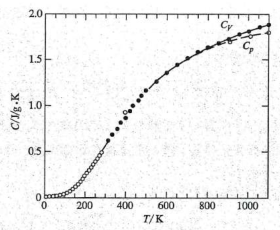
\includegraphics[height=43mm,keepaspectratio]{figures/fig_2_63_scan.png}
\par{\footnotesize 习题 2.63 图：金刚石的比热（原书图 2.24，原图摘录）}
\par{\footnotesize 原图注明来源：\textit{Semiconductor on NSM}。}
\end{center}
\endgroup
\vfill

\problem{2.64}
勒让德微分方程（Legendre's differential equation）为
\[
(1-x^2)\frac{\dd^2f}{\dd x^2}-2x\frac{\dd f}{\dd x}+l(l+1)f=0,
\]
这里 $l$ 是一些（非负）实数。
\begin{enumerate}
\item 假定存在一个幂级数解
\[
f(x)=\sum_{n=0}^{\infty}a_nx^n,
\]
给出常数 $a_n$ 的递推关系。
\item 论证除非这个级数被截断（只有当 $l$ 是整数时才会发生），方程的解在 $x=1$ 时将会发散。
\item 当 $l$ 是一个整数时，两个线性独立解中的一个级数序列会被截断（根据 $l$ 的奇偶不同，要么 $f_{\text{偶}}$，要么 $f_{\text{奇}}$），这些解称为勒让德多项式（Legendre polynomials）$P_l(x)$。利用递推关系求出 $P_0(x)$、$P_1(x)$、$P_2(x)$ 和 $P_3(x)$。答案用 $a_0$ 或者 $a_1$ 表示。
\end{enumerate}
\vfill
